\documentclass[11pt]{article}
\usepackage[a4paper,margin=2.4cm]{geometry}
\usepackage{amsmath,amssymb}
\usepackage{graphicx}
\usepackage{booktabs}
\usepackage{xcolor}
\usepackage{listings}
\usepackage[hidelinks]{hyperref}
\usepackage{caption}
\captionsetup{font=small}

\definecolor{codebg}{gray}{0.96}
\lstset{
  basicstyle=\ttfamily\small,
  backgroundcolor=\color{codebg},
  frame=single,
  framesep=4pt,
  breaklines=true,
  columns=fullflexible,
  keepspaces=true,
  showstringspaces=false,
}

\newcommand{\code}[1]{\texttt{\small #1}}

\title{\textbf{Time-dependent Hubbard magnetism and light-driven spin
currents in graphene nanoflakes}\\[4pt]
\large Implementation notes, figures, and physics summary}
\author{Working report}
\date{\today}

\begin{document}
\maketitle

\begin{abstract}
This report documents a set of changes to the tight-binding code for graphene
nanoflakes, in the order they were built. Three capabilities are covered:
(i) the self-consistent Hubbard (UHF) \emph{static} magnetic ground state that
underlies everything --- the ``frozen'' field; (ii) its \emph{time-dependent}
(TDUHF) extension that lets the magnetic order respond to an optical drive; and
(iii) a per-bond spin-current output that makes the spin flow visible in real
space. We explain the physics of each, the exact mean-field decomposition used
to avoid double counting, the numerical instability that a naive dynamic
implementation triggered and how it was cured, the configuration switches, and
the four analysis figures produced, with a reading of what each one tells us.
Throughout, the reference system is the $5\times5$ zigzag-edge triangular flake
(46 sites, sublattice imbalance $N_A-N_B=4$, Lieb spin $S=2$).
\end{abstract}

\tableofcontents

% ============================================================================
\section{Background and starting point}
The code evolves a spinful single-particle density matrix $\rho(t)$ (site basis,
ordering $[\uparrow_0\ldots\uparrow_{N-1},\downarrow_0\ldots\downarrow_{N-1}]$)
under a von~Neumann equation with a phenomenological relaxation
$-\tfrac{\gamma}{2}(\rho-\rho_0)$. Interactions enter at mean-field level:
\begin{itemize}
\item a \textbf{charge} Hartree term $V_{\rm ee}\,(\rho-\rho_0)$ that is
spin-blind and vanishes at equilibrium (it acts only on the \emph{induced}
density);
\item a self-consistent \textbf{Hubbard (UHF)} onsite exchange field that
produces the magnetic ground state. In the particle--hole-symmetric form the
onsite potential for spin $\sigma$ is
\begin{equation}
V_{i\sigma} = U\big(\langle n_{i,-\sigma}\rangle - \tfrac12\big).
\label{eq:uhf}
\end{equation}
\end{itemize}
The history below has three steps: the Hubbard field is first solved once and
held \textbf{frozen} to give the magnetic ground state (\S\ref{sec:frozen}); it
is then made \textbf{time-dependent} so the spin responds to the drive
(\S\ref{sec:tduhf}); and finally a \textbf{per-bond spin current} is added to see
the resulting spin flow in real space (\S\ref{sec:spincurrent}).

% ============================================================================
\section{Implementation 1: static (frozen) Hubbard/UHF magnetism}
\label{sec:frozen}
This is the foundation: the self-consistent magnetic ground state that all the
later work sits on. It was added first, and is ``frozen'' in the sense that it
is solved once and held fixed during the time evolution.

\subsection{Motivation}
Before this feature the model had \textbf{no equilibrium magnetism}. The up and
down blocks of $H_{\rm TB}$ were identical, so every eigenstate was
spin-degenerate, $\langle n_{i\uparrow}\rangle=\langle n_{i\downarrow}\rangle$
at every site, and the net moment was exactly zero. The only spin signal in the
whole simulation was the tiny ($\sim10^{-9}$) dynamical splitting from the
self-consistent induced magnetic field. Yet the zigzag triangle \emph{should} be
magnetic: its sublattice imbalance $N_A-N_B=4$ (25 $A$-sites, 21 $B$-sites)
produces \textbf{four zero-energy modes per spin}, and Lieb's theorem predicts a
ground state with total spin $S=|N_A-N_B|/2=2$.

\subsection{The Hubbard interaction at mean-field level}
Add the onsite Coulomb repulsion
$H=H_{\rm TB}+U\sum_i n_{i\uparrow}n_{i\downarrow}$. This term is quartic, so we
treat it in \textbf{unrestricted Hartree--Fock (UHF)}:
\begin{equation}
n_{i\uparrow}n_{i\downarrow}\approx
\langle n_{i\uparrow}\rangle n_{i\downarrow}
+ n_{i\uparrow}\langle n_{i\downarrow}\rangle
- \langle n_{i\uparrow}\rangle\langle n_{i\downarrow}\rangle,
\end{equation}
which reduces the interaction to the spin-dependent onsite potential
Eq.~\eqref{eq:uhf}, $V_{i\sigma}=U(\langle n_{i,-\sigma}\rangle-\tfrac12)$
(particle--hole-symmetric form, keeping the spectrum symmetric about $E=0$ at
charge neutrality so $\mu=0$). The up and down blocks are no longer identical:
if a site has more down- than up-electrons, the up level is pushed up and the
down level down, favouring further down-occupation --- the \textbf{Stoner
mechanism}. Above (here, any) critical $U$ the symmetric solution is unstable
and the flake develops a site-resolved magnetisation
$m_i=\tfrac12(n_{i\uparrow}-n_{i\downarrow})$, $S_z=\sum_i m_i$, arranged
antiferromagnetically (A-sublattice up, B down); the \emph{net} moment is carried
by the sublattice imbalance, giving $S_z=2$ exactly (Lieb).

\subsection{Self-consistency algorithm (\texttt{solve\_hubbard\_mft})}
$V_{i\sigma}$ depends on the occupations, which depend on $V_{i\sigma}$ --- solved
by iteration:
\begin{enumerate}
\item \textbf{Symmetry-breaking seed:} 2-colour the bond graph (BFS
$\to s_i=\pm1$) and start from a staggered guess
$n_{i\uparrow}=\tfrac12+\tfrac12 m_{\rm seed}s_i$,
$n_{i\downarrow}=\tfrac12-\tfrac12 m_{\rm seed}s_i$ (without a seed the symmetric
solution is a fixed point and no magnetism appears).
\item Build $H_{\rm MF}$ by adding $U(n_{i,-\sigma}-\tfrac12)$ to the diagonal.
\item Diagonalise; \textbf{fill} ($\rho_0$), transform to the site basis, read off
$n_{i\uparrow}=\rho_{ii}$, $n_{i\downarrow}=\rho_{N+i,N+i}$.
\item \textbf{Linear mix} $n\leftarrow(1-{\rm mix})\,n_{\rm old}+{\rm mix}\,n_{\rm new}$
(damps the Stoner feedback so the loop converges).
\item Converge when $\max_i|\Delta n_{i\sigma}|<$ tol ($10^{-8}$), else iterate
(up to 400).
\item Finalise: occupations, $V_{i\sigma}$, $m_i$, $S_z$, $\sum_i|m_i|$, and the
HOMO--LUMO \textbf{spin gap}.
\end{enumerate}

\subsection{Where the field lives (and a subtlety fixed during development)}
The converged $V_{i\sigma}$ is applied in \textbf{two} places so statics and
dynamics see the same magnet:
\begin{itemize}
\item \emph{Eigenproblem / $\rho_0$:} folded into a copy $H_{\rm c,eig}$, so the
eigenvalues and the initial density matrix are magnetic.
\item \emph{Time evolution:} kept \textbf{out} of the tight-binding base $H_0$
and re-added on the diagonal \emph{every step, in every branch} of
\code{build\_H\_for\_time}.
\end{itemize}
The second point matters: with \code{self\_consistent\_phase=true} the step
rebuilds $H$ from the hopping; if the exchange field lived only in $H_0$ that
rebuild would drop it, $\rho_0$ would not be stationary, and it would churn at
the $\sim$eV exchange scale --- wrong dynamics and a $\sim$4$\times$ slowdown from
tiny timesteps. Re-adding it every step keeps $\rho_0$ stationary.

\subsection{The value of $U$}
By default $U=v_{\rm ee}(0)\approx15.72$\,eV --- the onsite value of the
graphene-specific fitted Coulomb kernel, the same number sitting on the $V_{\rm ee}$
diagonal. It is overridable from the config (\code{hubbard\_U\_eV}); the TOML key
\code{coulomb\_onsite\_eV} is \emph{not} used for $U$.

\subsection{Configuration, outputs, validation}
\begin{lstlisting}
[features]
hubbard      = true    # self-consistent UHF magnetism (needs spin_on = true)
# hubbard_U_eV = 3.0    # optional U override in eV; unset/negative -> v_ee(0) ~ 15.7 eV
hubbard_seed = 0.5      # initial staggered moment for symmetry breaking
hubbard_mix  = 0.3      # linear mixing factor
\end{lstlisting}
Output: \code{magnetization.txt} (per-site \code{x y sublattice n\_up n\_dn m\_i}
plus a header with $U$, $S_{\rm total}$, $\sum|m_i|$, gap, iterations) and a
console summary. Validation on the reference flake: net $S_z=2.000$ exactly
(Lieb) at \emph{every} $U$; the moment magnitude and gap scale with $U$:
\begin{table}[h]
\centering
\begin{tabular}{lccc}
\toprule
$U$ (eV) & net $S_z$ & $\sum_i|m_i|$ & spin gap\\
\midrule
15.72 ($v_{\rm ee}(0)$) & 2 & 19.44 & 13.41\,eV\\
3.0  & 2 & 3.00 & 0.62\,eV\\
0.5  & 2 & 2.11 & 0.085\,eV\\
\bottomrule
\end{tabular}
\caption{The net $S=2$ is Lieb-protected and survives to tiny $U$ (the four
exactly-degenerate zero modes spin-polarise for any repulsion --- flat-band /
Stoner ferromagnetism); the antiferromagnetic background $\sum|m_i|$ and the gap
grow with $U$.}
\end{table}
Files: \code{Hamiltonians/hubbard.\{hpp,cpp\}} (new: \code{HubbardResult} +
\code{solve\_hubbard\_mft}); \code{main.cpp} (run the solver, fold into
$H_{\rm c,eig}$, write \code{magnetization.txt}); \code{DensityMatrix/Density.\{hpp,cpp\}}
(re-add the field every step); \code{params/*} (the knobs). Fully documented in
\code{HUBBARD\_FEATURE.md} \S1--9. With \code{hubbard=false} (default) none of
this runs.

% ============================================================================
\section{Implementation 2: time-dependent (TDUHF) spin channel}
\label{sec:tduhf}

\subsection{Goal and the key physical constraint}
We want the local moments to respond to the pulse. A crucial fact shapes
everything that follows: the Hamiltonian is \textbf{block-diagonal in spin}
(spin-conserving hopping, the diagonal UHF potential, a $\sigma_z$ Zeeman term,
and a spin-blind dipole drive). Therefore the \textbf{total}
$S_z=\tfrac12\sum_i(n_{i\uparrow}-n_{i\downarrow})$ is exactly conserved. Light
cannot change the net moment; it can only \emph{redistribute} spin between
sites, i.e.\ drive a transient \textbf{spin current} and local
(de)magnetisation at fixed $S_z$.

\subsection{Charge/spin decomposition (why there is no double counting)}
Writing the onsite mean field in terms of the total charge
$n_i=n_{i\uparrow}+n_{i\downarrow}$ and the moment
$m_i=n_{i\uparrow}-n_{i\downarrow}$, Eq.~\eqref{eq:uhf} splits into a
spin-blind \emph{charge} part and a spin-antisymmetric \emph{Stoner} part:
\begin{equation}
V_{i\sigma}=\underbrace{\tfrac{U}{2}\langle n_i\rangle}_{\text{charge}}
\;\mp\;\underbrace{\tfrac{U}{2}\langle m_i\rangle}_{\text{spin (Stoner)}},
\qquad (-\ \text{for}\ \sigma=\uparrow,\ +\ \text{for}\ \sigma=\downarrow).
\end{equation}
The charge part is the same physical object as the onsite ($v_{00}$) piece of
the classical Hartree term, which already couples to total charge and is
spin-blind. \textbf{We therefore keep the Hartree term exactly as it was} --- it
is the charge-channel restoring force. Only the \textbf{spin part}, which
couples to the moment and has \emph{no} Hartree counterpart, is made dynamic.
Because the two live in orthogonal channels, this cannot double-count.

\subsection{What is added each step}
On top of the frozen field we add the \textbf{live Stoner-exchange deviation}
\begin{equation}
\Delta V_{i,\uparrow/\downarrow}(t)=\mp\,\frac{U_{\rm spin}}{2}
\big(m_i(t)-m_i^{\rm eq}\big),\qquad
m_i(t)=\rho_{ii}^{\uparrow}(t)-\rho_{ii}^{\downarrow}(t).
\label{eq:stoner}
\end{equation}
Two design points matter:
\begin{itemize}
\item It is a \emph{functional of the instantaneous} $\rho(t)$, exactly like the
Hartree term, so the adaptive RK (dopri5) stages carry the self-consistency:
\textbf{no inner SCF loop}, $O(N)$ extra work per step.
\item We drive it with the moment \emph{deviation} $m_i(t)-m_i^{\rm eq}$ on top
of the frozen field, not the bare $m_i(t)$. This is the bare Stoner term plus a
constant, and it guarantees two things:
(a) \textbf{exact stationarity at any filling} --- graphene edges are not locally
half-filled, so anchoring on the frozen field keeps $\rho_0$ stationary for any
site occupation; (b) \textbf{$U_{\rm spin}\!\to\!0$ reproduces the frozen
dynamics exactly}. At exact half filling the two forms coincide.
\end{itemize}
$U_{\rm spin}$ (the Stoner coupling for the dynamic channel) is set separately
from the charge $U$; if unset it defaults to the charge $U$.

\subsection{The instability that a naive version triggered, and the cure}
A first attempt made the \emph{full} UHF field dynamic and, to avoid
double-counting the onsite Coulomb, deleted the onsite Hartree diagonal.
Stripping that diagonal removed the charge-channel restoring force and the
broken-symmetry state became \textbf{dynamically unstable} (a Thouless/RPA
instability of time-dependent mean-field theory around a saddle). With
\emph{zero drive}, the dipole grew exponentially from numerical noise
(e-folding $\sim 6$\,a.u.), reaching $\mathcal{O}(10)$, and the adaptive stepper
took $\sim$17$\times$ more steps. The instability was worst at small
$U$/small gap. The charge/spin split above cures it: the restoring force stays,
and only the (bounded) spin channel is made dynamic.

\subsection{Validation}
On the reference flake at $U=4.48$\,eV (the previously divergent case):
\begin{table}[h]
\centering
\begin{tabular}{lccc}
\toprule
zero-drive run & steps & $\max|{\rm dipole}|$ & $\max|{\rm spin\ induced}|$\\
\midrule
$U_{\rm spin}=U$ (full dynamic spin) & 1897 & $5\times10^{-14}$ & $3\times10^{-8}$\\
$U_{\rm spin}=0$ (reduces to frozen) & 1948 & $1\times10^{-8}$ & $5\times10^{-8}$\\
\emph{old scheme, same parameters} & $\sim$7700 & \emph{blows up to $-9.9$} & --\\
\bottomrule
\end{tabular}
\caption{Zero-drive stability. The ground state is now stationary to
solver-noise level; the previously divergent case is stable and $\sim$4$\times$
cheaper.}
\end{table}

\subsection{Configuration and files}
\begin{lstlisting}
[features]
hubbard          = true    # required: self-consistent UHF magnetic ground state
hubbard_dynamic  = true    # NEW: make the spin channel time-dependent (Stoner)
# hubbard_U_spin_eV = 4.48  # Stoner U for the dynamic spin channel;
                            #   if unset/negative -> uses the charge U
\end{lstlisting}
Files changed: \code{params/params.\{hpp,cpp\}} (new keys \code{hubbard\_dynamic},
\code{hubbard\_U\_spin\_eV}; derived \code{hub\_U}, \code{hub\_U\_spin},
\code{hub\_m\_eq}); \code{main.cpp} (store the couplings and the equilibrium
moment; console label); \code{DensityMatrix/Density.\{hpp,cpp\}} (solver carries
the new fields; \code{build\_H\_for\_time} adds the live Stoner deviation, the
classical Hartree left untouched). With \code{hubbard\_dynamic=false} the
behaviour is byte-for-byte identical to before. Documented in
\code{HUBBARD\_FEATURE.md} \S10.

% ============================================================================
\section{Implementation 3: per-bond spin current}
\label{sec:spincurrent}
The code previously wrote only the \emph{net} spin-current vector and the
\emph{charge} bond currents; there was no way to see spin flow in real space.
We added a per-bond spin current, the spin-difference analogue of the existing
charge bond current:
\begin{equation}
J^{\rm spin}_{\ell\ell'}=\frac{2e}{\hbar}\,\mathrm{Re}(H_{\ell\ell'})
\big[\mathrm{Im}\,\rho^{\uparrow}_{\ell\ell'}-\mathrm{Im}\,\rho^{\downarrow}_{\ell\ell'}\big],
\end{equation}
using the same Peierls-phase convention as the charge current (relevant for the
L2 self-consistent-phase runs). It is written every output step to
\code{J\_spin\_bond\_time\_evolution.txt} (one column per bond) whenever
\code{spin\_on} and the system is 2D. Implementation: \code{compute\_J\_bonds\_spin}
in \code{Density.cpp}, streamed through the existing \code{RhoObserver} /
\code{evolve\_rho\_over\_time} plumbing.

% ============================================================================
\section{What we measure, and the two drives}
\label{sec:observables}
Because total $S_z$ is conserved (\S\ref{sec:tduhf}), the informative spin
observables are \emph{not} the net moment (flat by construction) but:
\begin{itemize}
\item the \textbf{local induced moment} $m_i(t)-m_i^{\rm eq}$ (where spin sits);
\item the \textbf{staggered (N\'eel) moment}
$m_{\rm stag}(t)=\sum_i s_i\,m_i(t)$, with $s_i=\pm1$ the sublattice label
(the order parameter that can oscillate);
\item the \textbf{spin current} $J^{\rm spin}$ (net magnitude and per-bond).
\end{itemize}
Two drive shapes are available and give the two response regimes:
\begin{itemize}
\item \code{mode = "ddf"}: a near-instantaneous dipole kick $\to$
\textbf{linear response} (susceptibility / extinction $\sigma(\omega)$);
\item \code{mode = "time\_impulse"}: a finite Gaussian-envelope carrier pulse
$\to$ \textbf{nonlinear response} (high-harmonic generation, strong-field
dynamics).
\end{itemize}

% ============================================================================
\section{Figures and what they tell us}

\subsection{Control / validation: \texttt{plot\_hubbard\_dynamics.py}}
Plots $S_z(t)$, $\sum_i|m_i|(t)$ and the per-site moments $m_i(t)$ from the
induced spin diagonal. With \emph{zero drive} all three are flat to
$\sim10^{-8}$: the magnetic ground state is a genuine stationary state of the
TDUHF propagator. This is the sanity check behind the stability table above.

\subsection{The $U_{\rm spin}$ dial: \texttt{plot\_uspin\_dial.py}}
\begin{figure}[h]
\centering
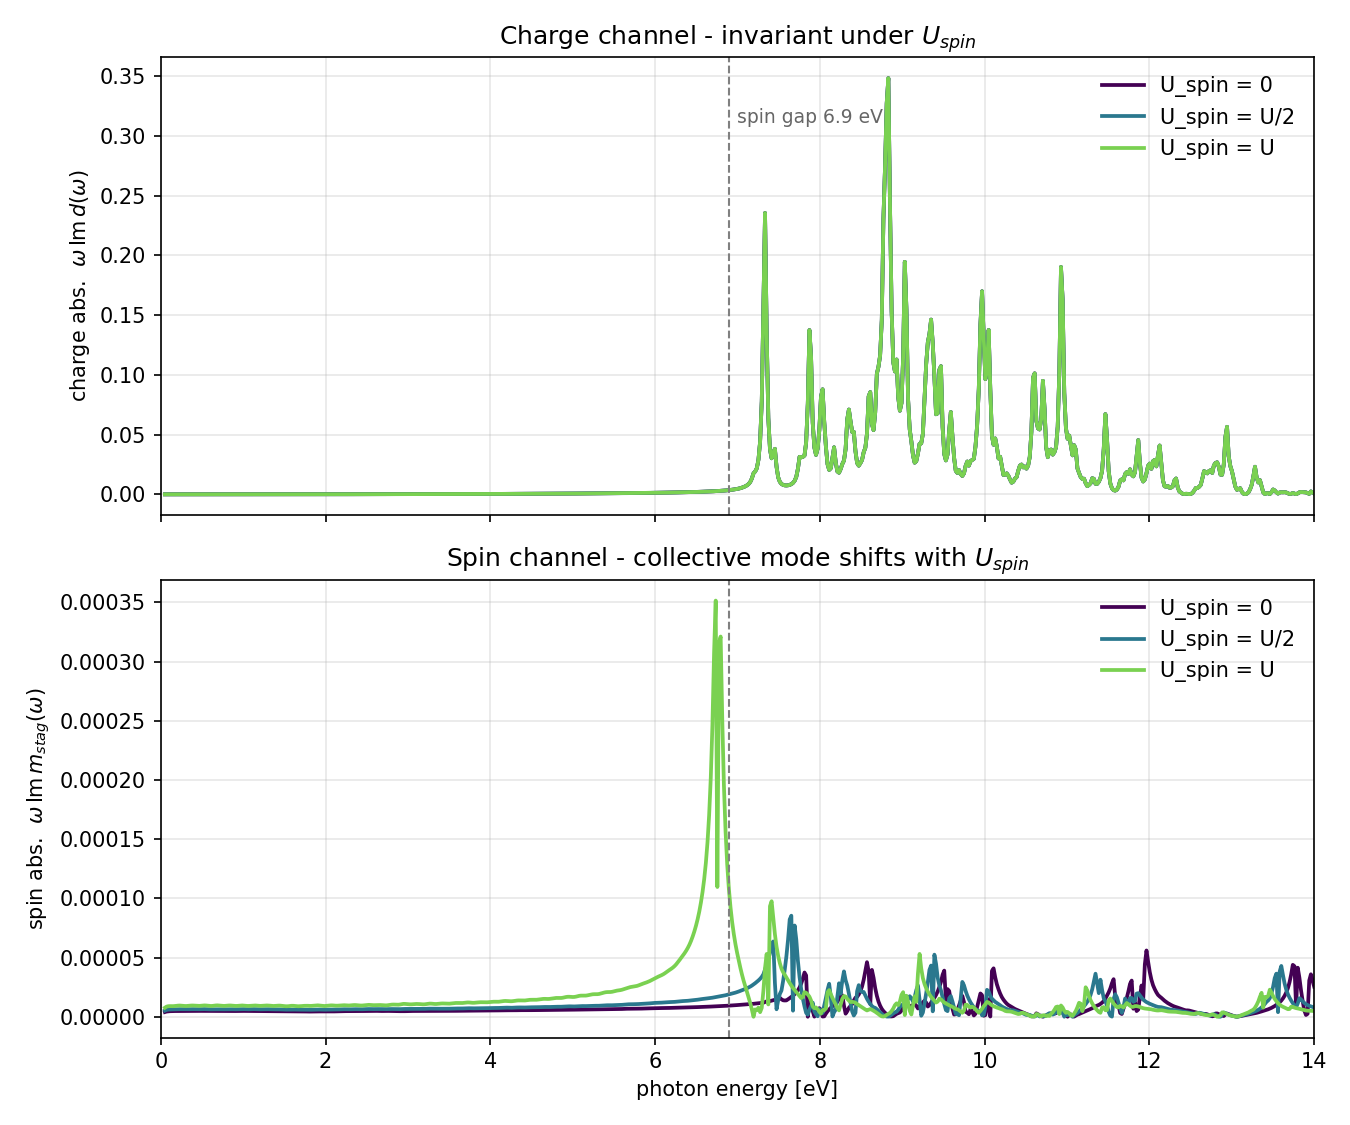
\includegraphics[width=0.92\linewidth]{figs/uspin_dial.png}
\caption{Linear-response (\code{ddf}) spectra for three Stoner couplings
$U_{\rm spin}=0,\,U/2,\,U$ at fixed charge $U$. \textbf{Top:} charge extinction
$\propto\omega\,\mathrm{Im}\,d(\omega)$ --- identical for all three (the charge
channel does not see $U_{\rm spin}$). \textbf{Bottom:} spin absorption
$\propto\omega\,\mathrm{Im}\,m_{\rm stag}(\omega)$. A sharp collective spin mode
appears at the spin gap ($\sim6.9$\,eV) and \emph{grows and sharpens with}
$U_{\rm spin}$; at $U_{\rm spin}=0$ there is no gap peak, only the bare
particle--hole background.}
\label{fig:dial}
\end{figure}
This figure is the direct demonstration that the dynamic spin channel is real:
the exchange coupling builds a collective (Stoner/RPA) spin mode that is absent
without it, while the charge channel is untouched --- clean channel separation.
Note the spectra are computed with the same Fourier convention as the built-in
$\sigma_{\rm ext}$ but out to a higher cutoff, and weighted by
$\omega\,\mathrm{Im}$ so the DC component is suppressed and the resonances stand
out (see \S\ref{sec:findings} for why the built-in \code{sigma\_ext.txt} alone,
capped at \code{omega\_cut\_off}, missed these peaks).

\subsection{The response matrix: \texttt{plot\_response\_matrix.py}}
\begin{figure}[h]
\centering
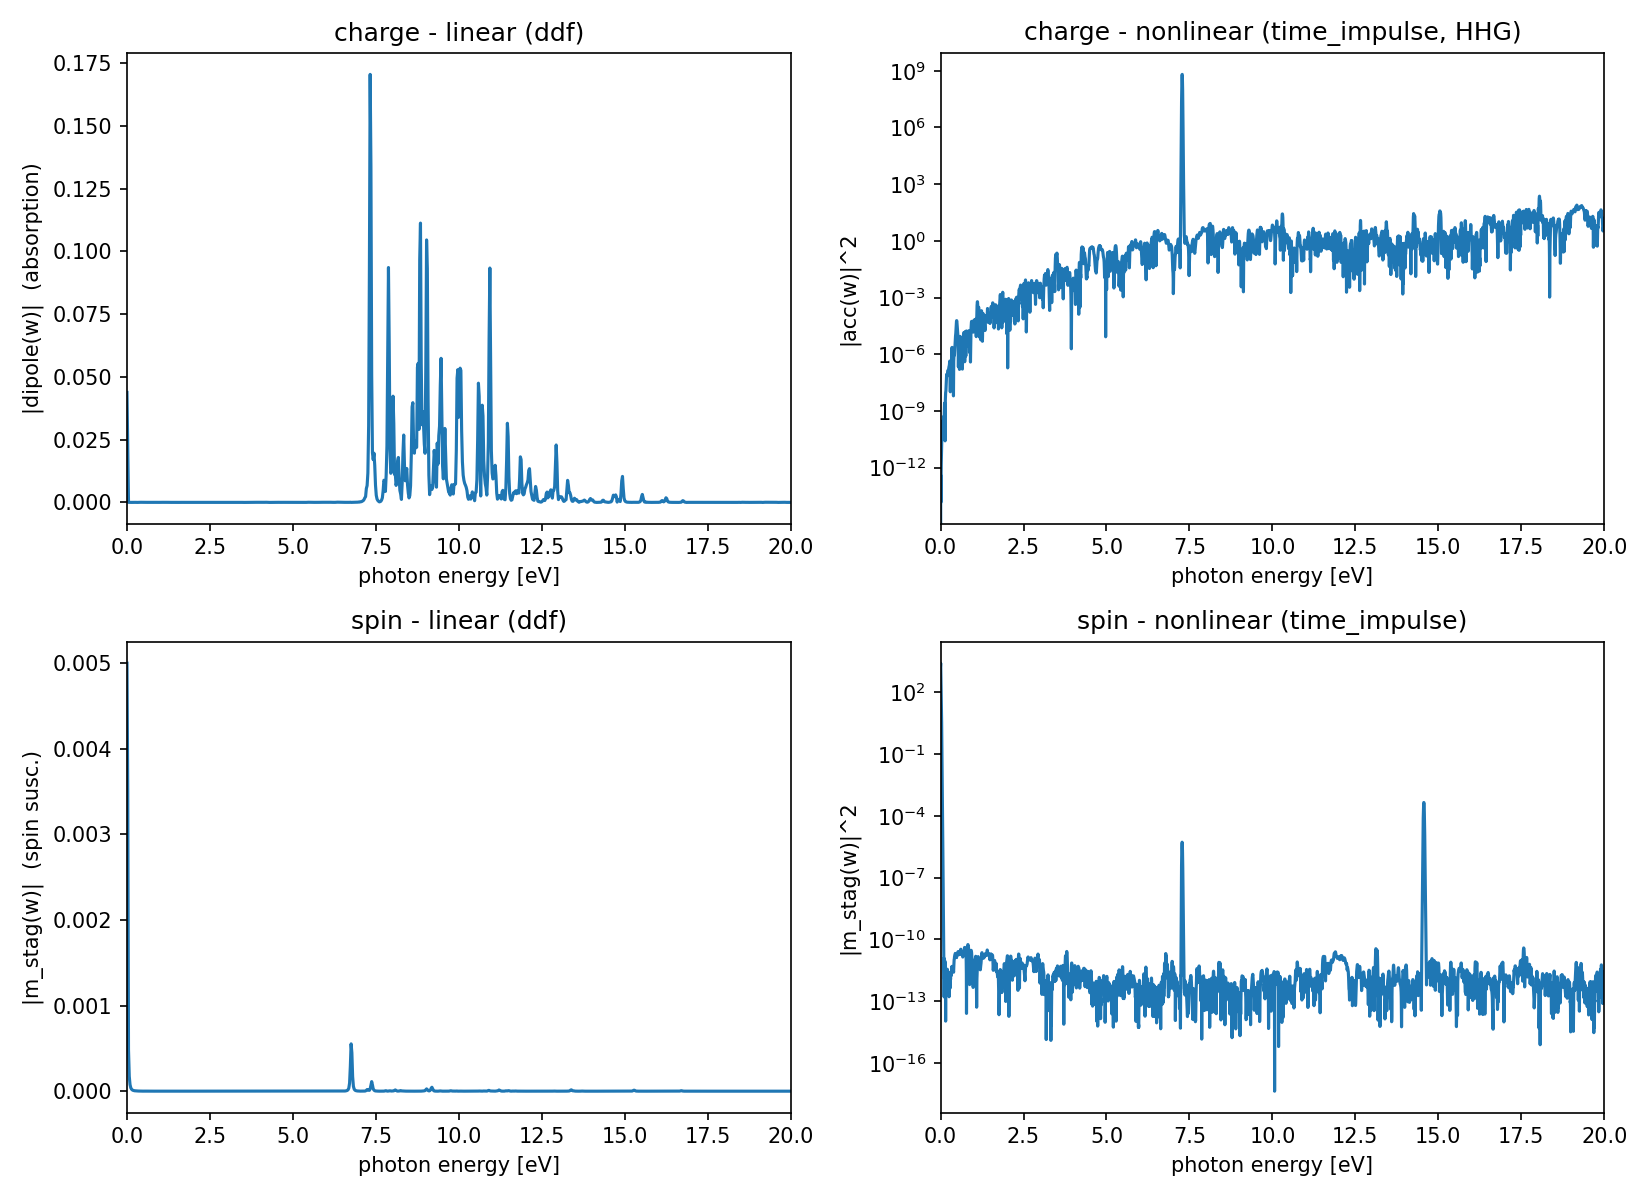
\includegraphics[width=0.92\linewidth]{figs/response_matrix.png}
\caption{Two drives (columns: linear \code{ddf} / nonlinear
\code{time\_impulse}) $\times$ two channels (rows: charge / spin) in one view.
Top row: charge absorption and charge HHG. Bottom row: the spin-channel
analogues from $m_{\rm stag}$.}
\label{fig:matrix}
\end{figure}
This is the ``map'' of the whole capability: the top row is the familiar charge
optics; the bottom row is what the dynamic Hubbard makes accessible --- a spin
response in both the linear (a collective mode) and nonlinear (spin harmonics)
regimes.

\subsection{Light-driven spin current in real space: \texttt{plot\_spin\_current\_realspace.py}}
\begin{figure}[h]
\centering
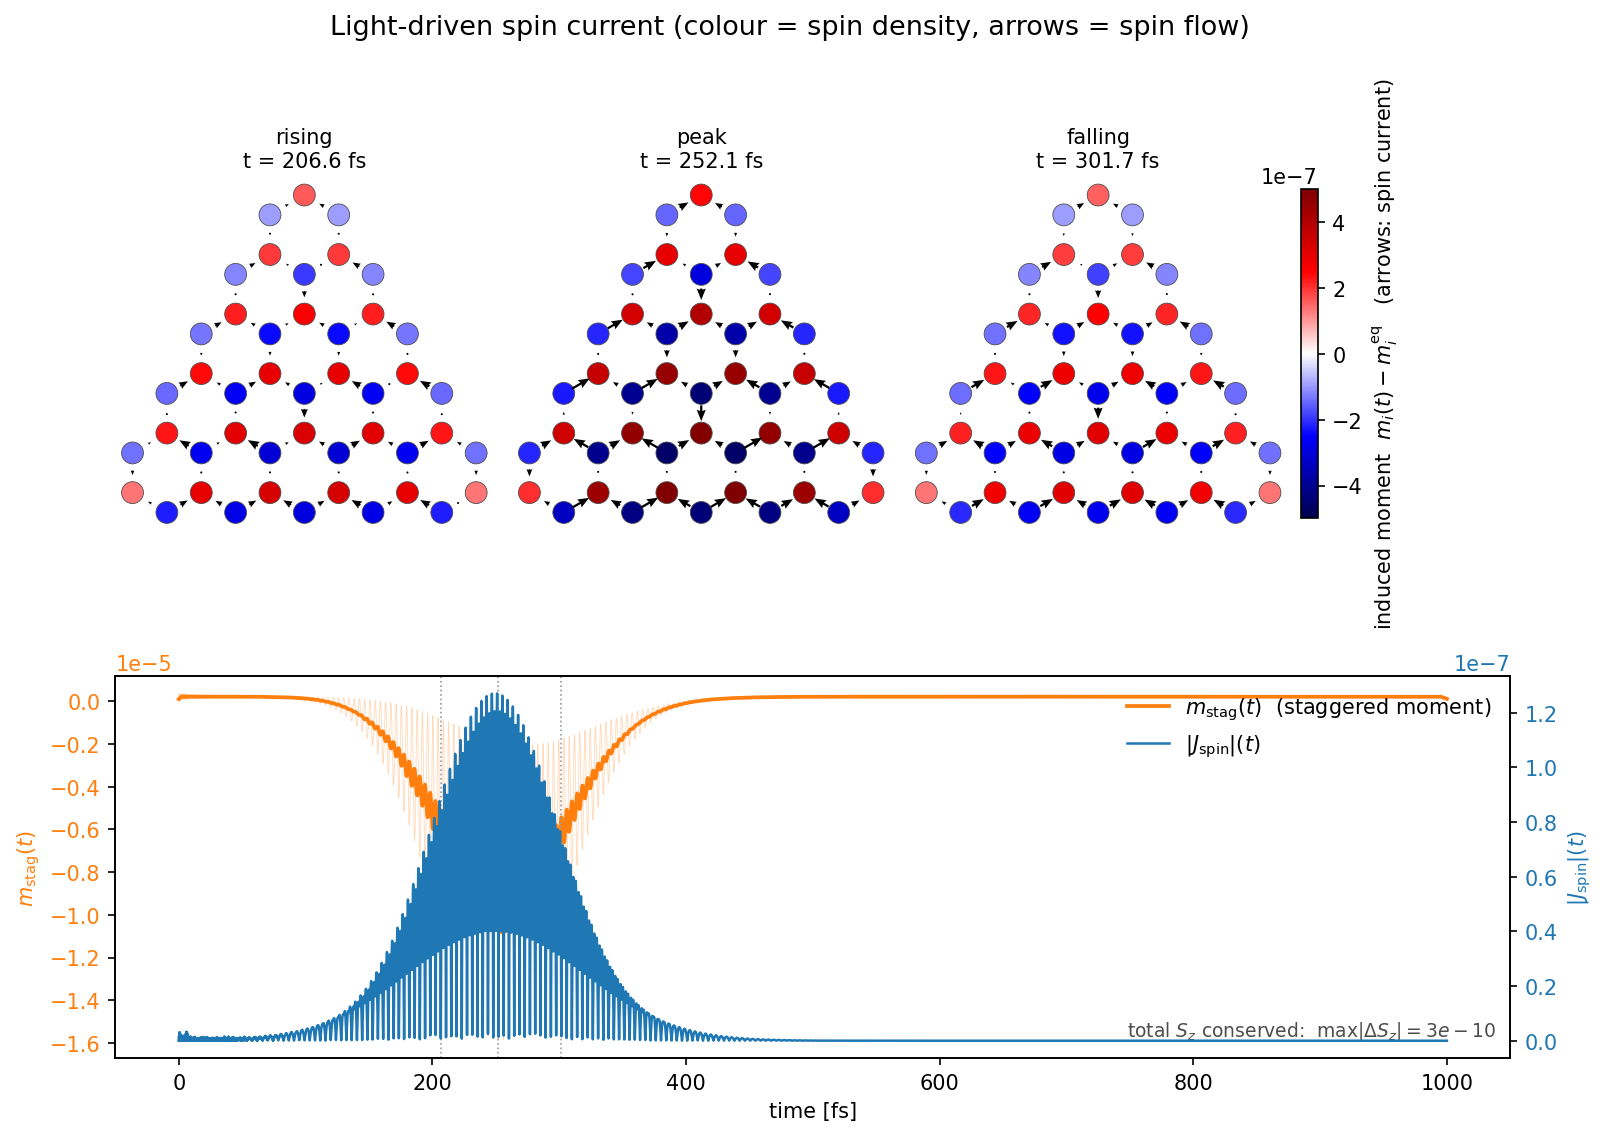
\includegraphics[width=0.98\linewidth]{figs/spin_current_realspace.png}
\caption{Strong-pulse (\code{time\_impulse}) run. \textbf{Top:} three snapshots
(rising / peak / falling of the response envelope). Node \emph{colour} is the
induced local moment $m_i(t)-m_i^{\rm eq}$ (where spin has piled up/depleted);
\emph{black arrows} on the bonds are the per-bond spin current $J^{\rm spin}$
(where and how fast spin flows). \textbf{Bottom:} the staggered moment
$m_{\rm stag}(t)$ (a transient demagnetisation of the N\'eel order) and the net
spin-current magnitude $|J_{\rm spin}|(t)$ on twin axes; the annotation confirms
total $S_z$ is conserved to $\sim10^{-8}$--$10^{-10}$.}
\label{fig:realspace}
\end{figure}
This is the physical picture the project is after: the pulse launches spin
currents that shuttle spin density between sublattices (colour texture) while
the net moment stays fixed --- ``redistribute, don't pump''. The arrows and the
colour are linked by continuity, $\partial_t m_i + \sum_{\rm bonds}J^{\rm spin}=0$.

% ============================================================================
\section{Physics findings}
\label{sec:findings}

\subsection{The gap and why the resonance moves so much with $U$}
The non-interacting zigzag triangle has \textbf{four zero-energy modes per spin}
(Lieb; $N_A-N_B=4$), i.e.\ the single-particle gap at $U=0$ is \emph{zero}.
Turning on $U$ spin-polarises and splits these modes symmetrically about $E=0$
by the exchange field; the eigenvalues cluster at $\pm3.4$--$3.7$\,eV for
$U=10.164$\,eV, giving a HOMO--LUMO gap of $6.9$\,eV. The gap is therefore
\textbf{entirely interaction-induced}, and tracks $\sim 2U\langle|m_i|\rangle$:
\begin{table}[h]
\centering
\begin{tabular}{lcccc}
\toprule
$U$ (eV) & $\sum_i|m_i|$ & $\langle|m|\rangle$ & $2U\langle|m|\rangle$ & measured gap\\
\midrule
4.48   & 4.03 & 0.088 & 0.79\,eV & 1.11\,eV\\
10.164 & 15.05 & 0.327 & 6.65\,eV & 6.89\,eV\\
\bottomrule
\end{tabular}
\caption{The gap is set by the self-consistent exchange splitting. Both $U$ and
the moment grow together, so the optical resonance shifts \emph{faster} than
linearly in $U$ --- a large shift is expected, and it appears for the frozen
field too because it is a ground-state property.}
\end{table}
Two cautions: (i) this is a mean-field \textbf{Slater} (symmetry-broken) gap,
\emph{not} a true Mott gap --- UHF systematically overestimates moments and
gaps, so the magnitudes should not be read quantitatively; (ii) in the static
ground state there is no double screening --- the gap comes purely from the UHF
field, the induced Hartree being zero at equilibrium.

\subsection{Collective spin mode}
The bottom panel of Fig.~\ref{fig:dial} shows the payoff of the dynamic channel:
a collective spin resonance at the gap whose weight is controlled by
$U_{\rm spin}$. It is the time-dependent-mean-field (RPA) mode of the
broken-symmetry state, absent when the spin channel is frozen.

\subsection{Spin transport at fixed $S_z$}
Fig.~\ref{fig:realspace} shows the central result enabled by both
implementations together: an optical pulse drives real-space spin currents and a
transient reduction of the N\'eel order, with the total spin exactly conserved.

% ============================================================================
\section{How to reproduce}
Reference flake: \code{configs/graphene\_zigzag\_triangle.toml}
($5\times5$ zigzag triangle, \code{spin\_on=true}, \code{hubbard=true},
\code{hubbard\_dynamic=true}). Suggested run matrix:
\begin{table}[h]
\centering
\begin{tabular}{lccl}
\toprule
run & drive & $U_{\rm spin}$ & purpose / figure\\
\midrule
A & \code{ddf} & 0 & linear baseline (Fig.~\ref{fig:dial}, Fig.~\ref{fig:matrix})\\
B & \code{ddf} & $U/2,\,U$ & $U_{\rm spin}$ dial (Fig.~\ref{fig:dial})\\
C & \code{time\_impulse} & $U$ & nonlinear + real-space spin current
(Fig.~\ref{fig:matrix}, Fig.~\ref{fig:realspace})\\
\bottomrule
\end{tabular}
\end{table}

\noindent Practical notes:
\begin{itemize}
\item The \code{ddf} runs are cheap; only \code{time\_impulse} runs are long.
\item Keep $U$ in the stable regime; very small gaps stress the mean-field
dynamics.
\item The adaptive solver writes non-uniform (and occasionally duplicated) time
stamps --- all spectral scripts resample onto a uniform grid before FFT.
\item For the built-in \code{sigma\_ext.txt} to contain the resonances, set
\code{omega\_cut\_off} above the gap (the analysis scripts compute their own
spectra to a higher cutoff regardless).
\item \code{plot\_spin\_current\_realspace.py} needs
\code{J\_spin\_bond\_time\_evolution.txt}, i.e.\ a run made \emph{after} the
per-bond spin-current change.
\end{itemize}

\paragraph{Analysis scripts (all take a folder path at the top).}
\code{plot\_hubbard\_dynamics.py} (control), \code{plot\_uspin\_dial.py}
(Fig.~\ref{fig:dial}), \code{plot\_response\_matrix.py} (Fig.~\ref{fig:matrix}),
\code{plot\_spin\_current\_realspace.py} (Fig.~\ref{fig:realspace}).

\end{document}
